\section{Evelyn Paxos}
In this section, we first describe \emph{how} Evelyn Paxos works
(\secref{EvelynPaxos/Overview}) and then \emph{why} it is safe
(\secref{EvelynPaxos/SafetyProof}). We then discuss liveness
(\secref{EvelynPaxos/Liveness}) and non-linearizable reads
(\secref{EvelynPaxos/NonLinearizableReads}).

\subsection{Overview}\seclabel{EvelynPaxos/Overview}
The Paxos Quorum Read protocol (PQR) allows reads to bypass the leader and
execute on a single replica. However, a client executing a read must contact at
least a majority of a fixed set of $2f+1$ acceptors. Thus, the acceptors are a
bottleneck that limits the read throughput of the protocol. Moreover, if we
increase the number of replicas in a PQR deployment to increase \emph{read}
throughput, we increase the communication load on the leader and decrease the
deployment's \emph{write} throughput.

Compartmentalized MultiPaxos, on the other hand, deploys multiple acceptor
groups and can scale up the number replicas without impacting write throughput.
Compartmentalized MultiPaxos, however, does not distinguish reads from writes.
All state machine commands are sent to the leader, placed in the replicated
log, and executed by all replicas.

\defword{Evelyn Paxos} is the straightforward combination of Compartmentalized
MultiPaxos and PQR. By combining the strengths of the two protocols, Evelyn
Paxos achieves scalable, linearizable reads that bypass the leader and execute
at a single replica.

An Evelyn Paxos deployment is identical to a Compartmentalized MultiPaxos
deployment, and both protocols process writes in exactly the same way. Evelyn
Paxos reads are very similar to PQR reads with a few minor differences.

Concretely, to perform a read, an Evelyn Paxos client sends \msg{MaxSlotA}{}
messages to at least a majority of acceptors in any single acceptor group. The
client does \emph{not} have to contact all of the acceptor groups, just a
single one.
%
When an acceptor $a_i$ receives a \msg{MaxSlotA}{} request from a client, it
replies with a \msg{MaxSlotB}{s_i} message, where $s_i$ is the largest log
entry in which $a_i$ has voted, or $0$ if $a_i$ has not yet voted in any log
entry.

The client waits to receive \msg{MaxSlotB}{s_i} replies from at least a
majority of the acceptors in a single group and then computes $s_\text{max}$ as
the maximum received $s_i$. Let $m$ be the number of acceptor groups. The
client computes $s = s_\text{max} + m - 1$ and then sends a \msg{Read}{x, s}
message to any replica, with the read command $x$ and the slot $s$.
%
When a replica receives a \msg{Read}{x, s} message, it waits until it has
executed the write in log entry $s$, then executes $x$, and finally returns the
result of executing $x$ back to the client. This is illustrated in
\figref{EvelynPaxos}.

Note that a replica can service a \msg{Read}{x, s} message even if it has
already executed writes in log entries larger than $s$. That is, $x$ does not
have to read from $s$ exactly; it just has to read from a log entry at least as
large as $s$. We also re-emphasize that reads wait for writes. We discuss the
liveness and performance implications of this later.

{% Processes.
\tikzstyle{proc}=[draw, circle, thick, inner sep=2pt]
\tikzstyle{igproc}=[draw=gray, text=gray]
\tikzstyle{client}=[proc, fill=clientcolor!25]
\tikzstyle{proposer}=[proc, fill=proposercolor!15]
\tikzstyle{proxyleader}=[proc, fill=proxyleadercolor!15]
\tikzstyle{acceptor}=[proc, fill=acceptorcolor!25, font=\scriptsize]
\tikzstyle{replica}=[proc, fill=replicacolor!25]

% Process labels.
\tikzstyle{proclabel}=[inner sep=0pt, align=center, font=\footnotesize]

% Components.
\tikzstyle{component}=[draw, thick, flatgray, rounded corners]

% Messages and communication.
\tikzstyle{comm}=[-latex, thick]
\tikzstyle{commnum}=[fill=white, inner sep=0pt]

\begin{figure}[ht]
  \centering
  \begin{tikzpicture}[xscale=1.5]
    % Processes.
    \node[client] (c1) at (0, 2) {$c_1$};
    \node[client] (c2) at (0, 1) {$c_2$};
    \node[client] (c3) at (0, 0) {$c_3$};
    \node[proposer, igproc] (p1) at (1, 1.5) {$p_1$};
    \node[proposer, igproc] (p2) at (1, 0.5) {$p_2$};
    \node[proxyleader, igproc] (pl1) at (2, 2) {$l_1$};
    \node[proxyleader, igproc] (pl2) at (2, 1) {$l_2$};
    \node[proxyleader, igproc] (pl3) at (2, 0) {$l_3$};
    \node[acceptor] (a01) at (3, 2) {$a^0_1$};
    \node[acceptor] (a02) at (3.5, 2) {$a^0_2$};
    \node[acceptor] (a03) at (4, 2) {$a^0_3$};
    \node[acceptor] (a11) at (3, 0) {$a^1_1$};
    \node[acceptor] (a12) at (3.5, 0) {$a^1_2$};
    \node[acceptor] (a13) at (4, 0) {$a^1_3$};
    \node[replica] (r1) at (5, 2) {$r_1$};
    \node[replica] (r2) at (5, 1) {$r_2$};
    \node[replica] (r3) at (5, 0) {$r_3$};

    % Labels.
    \crown{(p1.north)++(0,-0.15)}{0.333}{0.25}
    \node[proclabel] (clients) at (0, 3) {Clients};
    \node[proclabel, text=gray] (proposers) at (1, 3) {$f+1$\\Proposers};
    \node[proclabel, text=gray] (proxyleaders) at (2, 3) {$\geq f+1$\\Proxy\\Leaders};
    \node[proclabel] (acceptors) at (3.5, 3) {$\geq 1$ group of \\$2f+1$ Acceptors};
    \node[proclabel] (replicas) at (5, 3) {$\geq f+1$\\Replicas};
    \halffill{clients}{clientcolor!25}
    \quarterfill{proposers}{proposercolor!25}
    \quarterfill{proxyleaders}{proxyleadercolor!25}
    \quarterfill{acceptors}{acceptorcolor!25}
    \quarterfill{replicas}{replicacolor!25}

    % Communication.
    \draw[comm, bend right=20] (c2) to node[commnum]{1} (a11);
    \draw[comm, bend left=10] (c2) to node[commnum]{1} (a12);
    \draw[comm, bend left=35] (a11) to node[commnum]{2} (c2);
    \draw[comm, bend left=5] (a12) to node[commnum]{2} (c2);
    \draw[comm, bend left=7] (c2) to node[commnum]{3} (r1);
    \draw[comm, bend left=7] (r1) to node[commnum]{4} (c2);
  \end{tikzpicture}
  \caption{%
    An example Evelyn Paxos read. Proposers and proxy leaders are grayed
    because they are not involved in reads. An Evelyn Paxos write is identical
    to a Compartmentalized MultiPaxos write; see
    \figref{MultiPaxosMoreReplicasDiagram}.
  }%
  \figlabel{EvelynPaxos}
\end{figure}
}

Because an Evelyn Paxos read involves only a single acceptor group and a single
replica, we can scale up the number of acceptor groups and replicas to increase
the protocol's aggregate read throughput.

% Recall that Paxos Quorum Reads does not allow for high read throughput because
% the acceptors or replicas eventually become a bottleneck. With Evelyn Paxos,
% however, both the acceptors and the replicas are scalable. Thus, by increasing
% the number of acceptor groups and replicas, read throughput increases without
% any bottlenecks.

\subsection{Safety Proof}\seclabel{EvelynPaxos/SafetyProof}
We now prove that Evelyn Paxos is linearizable. We provide a proof not only to
convince you that the protocol is safe, but also to help build some intuition
on the protocol. For example, the proof should hopefully make clear why Evelyn
Paxos requires a $+\ m - 1$ term that PQR does not.

\newcommand{\complete}{\text{complete}}
\begin{proof}
  Let $H$ be an arbitrary history permitted by Evelyn Paxos. To prove that
  Evelyn Paxos is linearizable, we must extend $H$ to a history $H'$ such that
  $\complete(H')$ is equivalent to a sequential history that respects $<_H$.

  Recall that extending $H$ to $H'$ is sometimes necessary because of
  situations like the one shown in \figref{WhyExtendHistory}. This example
  involves a single register with an initial value of 0. $c_1$ issues a request
  to write the value of 1, but has not yet received a response. $c_2$ issues a
  read request and receives the value 1. If we do not extend the history to
  include a response to $c_1$'s write, then there will not exist an equivalent
  sequential history.

  {\begin{figure}[ht]
  \centering
  \begin{tikzpicture}
    \drawclients{2}{3.5};
    \pendingoperation{1}{0}{3}{$w(1)$}
    \operation{2}{1}{2}{$r()$}{$1$}
  \end{tikzpicture}
  \caption{A motivating example of history extension}\figlabel{WhyExtendHistory}
\end{figure}
}

  So, which operations should we include in $H'$? Let $k$ be the largest log
  index written in or read from in $\complete(H)$. First note that for every
  index $0 \leq i \leq k$, there exists a (potentially pending) write in $H$
  that has been chosen in index $i$. Why?  Well, Evelyn Paxos, like MultiPaxos,
  executes commands in log order, so a write at index $k$ can only complete
  after all writes with smaller indices have been chosen (and executed by some
  replica). Similarly, if a read operation reads from slot $k$, then the write
  in slot $k$ must have been executed, so again all writes with smaller indices
  have also been chosen.
  %
  We extend $H$ to history $H'$ by including responses for all pending write
  invocations with indices $0 \leq i \leq k$. The responses are formed by
  executing the $k + 1$ commands in log order.

  For example, consider the history $G$ shown in \figref{ExtendExample}. $w_i$
  represents a write chosen in log index $i$, $r_i$ represents a read operation
  that reads from slot $i$, $w_?$ represents a pending write which has not been
  chosen in any particular log index, and $r_?$ represents a pending read.
  %
  $\complete(G)$ includes $w_1$ and $r_2$, so here $k=2$ and we must include
  all writes in indices $0$, $1$, and $2$. That is, we extend $G$ to complete
  $w_0$ and $w_2$. $w_4$ is left pending, as is $w_?$ and $r_?$. Also note
  that we could not complete $w_4$ even if we wanted to because there is no
  $w_3$.

  {\begin{figure}[ht]
  \begin{tikzpicture}[yscale=0.75]
    \drawclients{5}{7.5}
    \pendingoperation{1}{0}{7}{$w_0$}
    \operation{2}{1}{2}{$w_1$}{}
    \pendingoperation{2}{3}{7}{$w_2$}
    \operation{3}{2.5}{3.5}{$r_2$}{}
    \pendingoperation{3}{4}{7}{$w_4$}
    \operation{4}{4}{5}{$r_2$}{}
    \pendingoperation{4}{6}{7}{$w_?$}
    \pendingoperation{5}{2}{7}{$r_?$}
  \end{tikzpicture}
  \caption{%
    An example history $G$. Responses are not shown, as they are not important
    for this example.
  }\figlabel{ExtendExample}
\end{figure}
}

  Now, we must prove that (1) $\complete(H')$ is equivalent to some legal
  sequential history $S$, and (2) $<_H$ respects $<_S$. We let $S$ be the
  sequential history formed from executing all writes in log order and from
  executing every read from index $i$ after the write in index $i$.
  %
  If there are multiple reads from index $i$, the reads are ordered in an
  arbitrary way that respects $<_H$. For example, the history $G$ in
  \figref{ExtendExample} has the sequential history $S_G$ shown in
  \figref{ExampleS}. Note that $c_4$'s read comes after $c_3$'s read. This is
  essential because we must respect $<_G$. If the two reads were concurrent in
  $G$, they could be ordered arbitrarily in $S_G$.

  {\begin{figure}[ht]
  \centering
  \begin{tikzpicture}[yscale=0.75]
    \drawclients{4}{7.5}
    \operation{1}{0}{1}{$w_0$}{}
    \operation{2}{1.5}{2.5}{$w_1$}{}
    \operation{2}{3}{4}{$w_2$}{}
    \operation{3}{4.5}{5.5}{$r_2$}{}
    \operation{4}{6}{7}{$r_2$}{}
  \end{tikzpicture}
  \caption{A linearization $S_G$ of the history in $G$ \figref{ExtendExample}}%
  \figlabel{ExampleS}
\end{figure}
}

  To prove (1) and (2), we show that if two distinct operations $x$ and $y$
  that write to (or read from) log indices $i$ and $j$ are related in
  $H$---i.e. $x <_H y$, or $x$ finishes before $y$ begins---then $i \leq j$. We
  perform a case analysis on whether $x$ and $y$ are reads or writes.

  \begin{itemize}
    \item \textbf{$x$ and $y$ are both writes:}
      At the time $x$ completes in index $i$, all commands in indices less than
      $i$ have been chosen because Evelyn Paxos executes commands in log order.
      Thus, when $y$ later begins, it cannot be chosen in a log entry less than
      $i$, since every log entry implements consensus. Thus, $i < j$.

    \item \textbf{$x$ and $y$ are both reads:}
      When $x$ completes, command $i$ has been chosen. So have commands $i-1$,
      $i-2$, $i-3$, $\ldots$, $i-(m-1)$. Each of these $m$ commands were chosen
      by a different acceptor group.
      %
      When $y$ begins, it sends \msg{MaxSlotA}{} messages to some majority
      $M_1$ of some acceptor group. Assume this acceptor group chose log entry
      $i - j$ for some $0 \leq j \leq m-1$.  Because log entry $i-j$ was chosen
      by the acceptor group, at least a majority $M_2$ of the acceptor group
      voted for log entry $i-j$.  Any two majorities intersect, including $M_1$
      and $M_2$.  Thus, the client executing $y$ will receive a
      \msg{MaxSlotB}{s_i} response from some acceptor in $M_2$ with $s_i \geq
      i-j$. Therefore, $s_\text{max} \geq i - j$ and
      \[
        s = s_\text{max} + m - 1
          \geq i - j + m - 1
          \geq i - (m-1) + (m - 1)
          = i
      \]
      Therefore, $y$ is guaranteed to read from some $j \geq s = i$.

    \item \textbf{$x$ is a read and $y$ is a write:}
      When $x$ completes, all commands in indices $i$ and smaller have been
      chosen. By the first case above, $y$ must be chosen in some index $j >
      i$.

    \item \textbf{$x$ is a write and $y$ is a read:}
      When $x$ completes, command $i$ has been chosen. If $i \leq m-1$, then $j \geq
      i$ immediately since $i = i' + m - 1$ for some natural number $i'$.
      Otherwise, $i > m - 1$. $i$ has been chosen, and so has $i-1$ through
      $i-(m-1)$, each by a different acceptor group.
      %
      As with the second case above, when $y$ begins it will contact an
      acceptor group with a largest chosen value at least as large as $i-(m-1)$
      and will subsequently read from at least $i$.
  \end{itemize}

  From this, (1) is immediate since every client's operations are in the same
  order in $H'$ and in $S$. (2) holds because $S$ is ordered by log index with
  ties broken respecting $<_H$, so if $x <_H y$, then $i \leq j$ and $x <_S y$.
\end{proof}

\subsection{Ensuring Liveness}\seclabel{EvelynPaxos/Liveness}
When an Evelyn Paxos replica receives a read request at index $s$, it cannot
perform the read until it has executed the write in log entry $s$. The duration
of time that the replica must wait depends on the throughput of writes being
sent to the Evelyn Paxos deployment. In the extreme, if no writes are being
proposed, then the replica could stall, waiting forever to execute log entry
$s$, even though no command has been or will be proposed to fill it. This is a
liveness violation.

Fortunately, this problem is easy to fix. An Evelyn Paxos leader periodically
proposes a noop in the log. This ensures that all reads are eventually
serviced. The period at which an Evelyn Paxos leader proposes noops is a
tunable parameter. For workloads with few writes or no writes, the leader
should propose noops often to decrease read latency. For workloads with high
write throughputs, however, the leader does not have to propose noops often if
at all.

\subsection{Non-Linearizable Reads}\seclabel{EvelynPaxos/NonLinearizableReads}
\TODO[mwhittaker]{Write.}
